%Language: LaTeX
%Script: Florida_warming.tex
%Des: Is Florida warmer?

\documentclass{article}

%\date{Oct, 2021}

% Language setting
% Replace `english' with e.g. `spanish' to change the document language
\usepackage[english]{babel}

% Set page size and margins
% Replace `letterpaper' with`a4paper' for UK/EU standard size
\usepackage[letterpaper,top=2cm,bottom=2cm,left=3cm,right=3cm,marginparwidth=1.75cm]{geometry}

% Useful packages
\usepackage{amsmath}
\usepackage{graphicx}
\graphicspath{{../sandbox/}}
\usepackage[colorlinks=true, allcolors=blue]{hyperref}
\usepackage{float}

\title{Is Florida getting warmer?}
\author{Congjia Chen (Congjia.Chen21@imperial.ac.uk)}

\begin{document}
\maketitle

\section{Results and Discussion}

\subsection{Coefficient Efficient distribution}
After repeating 10,000 times, we have 10001 correlation coefficients (10000 random and 1 raw). See density distribution below \ref{fig:Density_plot}:
The blue dash line demonstrated the correlation coefficients of the raw data set. The 10000 random correlation coefficient shows random distribution. Approximately no random correlation coefficients are bigger than the raw one. The correlation coefficient of the raw data set is 0.53317.
\begin{figure}[H]
\centering
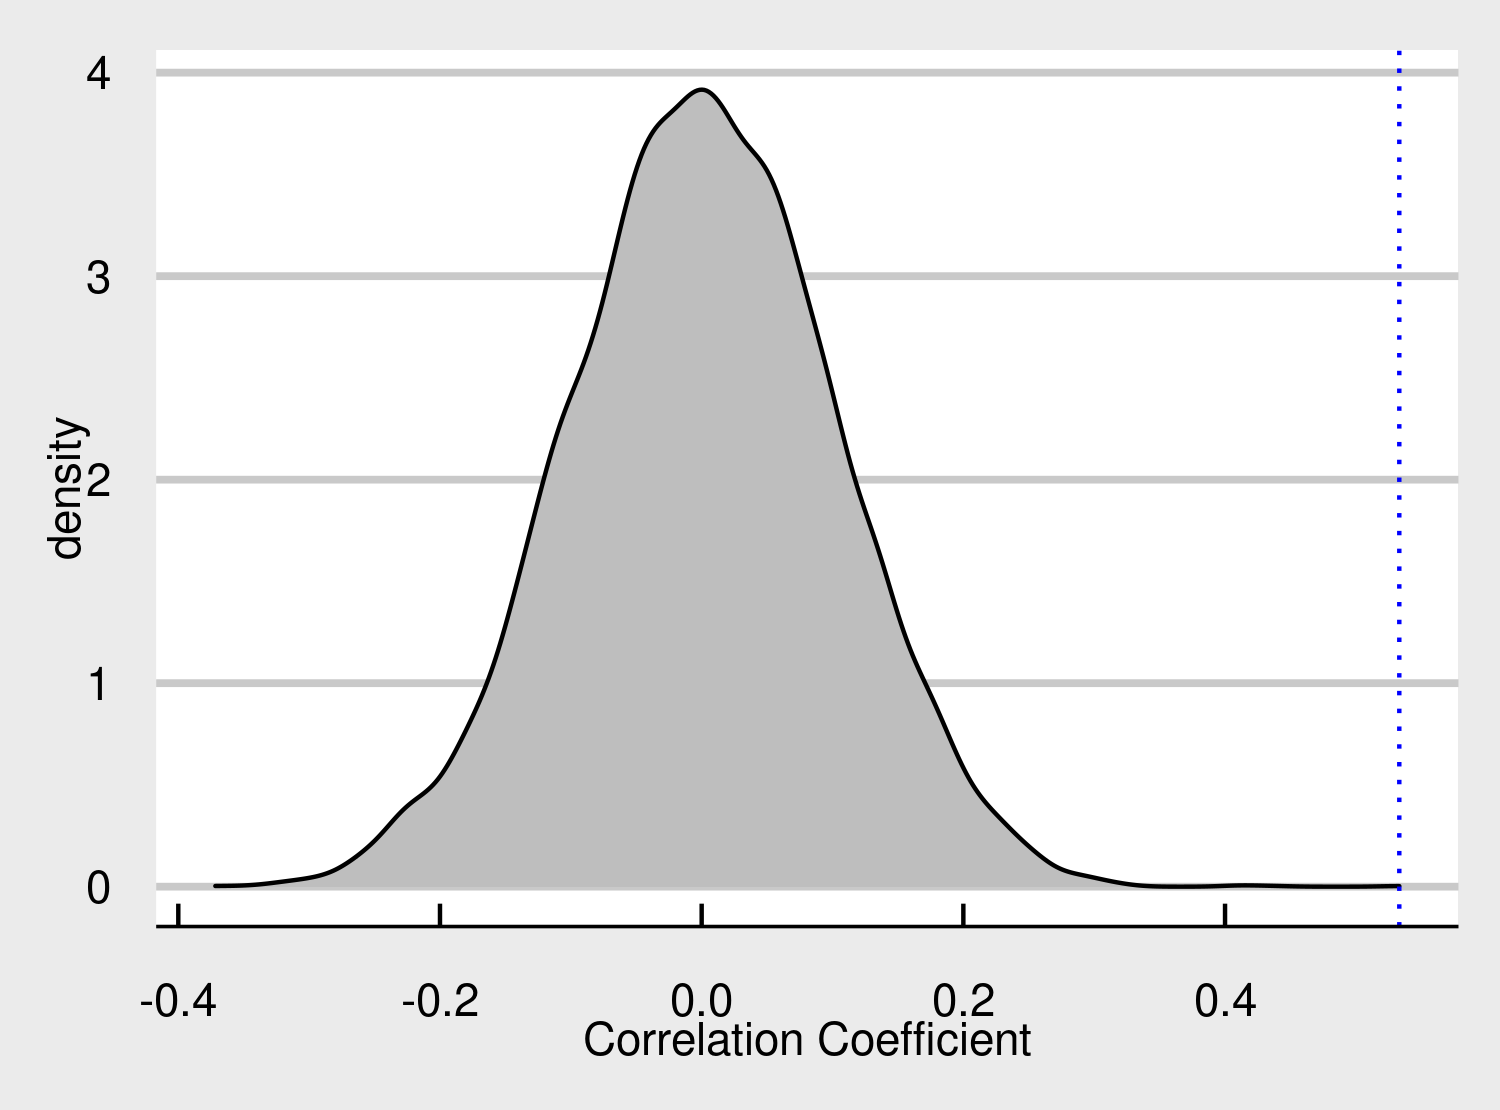
\includegraphics[width=0.7\textwidth]{Density_plot.png}
\caption{\label{fig:Density_plot}The Density plot of Correlation Coefficient}
\end{figure}

\subsection{Estimation of \texorpdfstring{$\mathit{p}$}{}-value}
The approximate \textit{p}-value could be represented by the fraction of the random correlation coefficients whose absolute value were greater than the observed one. The fraction is 0.00000.
The correlation coefficient is 0.53317, showing that there is a relatively weak positive correlation between the temperatures of one year and its successive year. In terms of the statistical significance, we use a permutation analysis, by generating a distribution of random correlation coefficients and compare our observed coefficient with this random distribution. Fraction of the random correlation coefficients whose absolute value were greater than the observed one is 0, indicating the significance statistically.

\section{Supplement}
  All codes can be found in Florida.R, please visit the code in \href{https://github.com/nedchen2/CMEECourseWork/blob/master/week3/code/Florida_warming.R}{my repository}.
\end{document}